\section{2016-10-8}
\subsection{ICP algorithm test}
I found and tested a source code of the ICP algorithm on a point cloud. I firstly transformed the initial point cloud (white in Fig~\ref{icp_fish}) to get a transformed point cloud (green in Fig~\ref{icp_fish}) with a randomly selected Rotation Matrix $\textbf{R}$ and a Translation Matrix $\textbf{T}$. And then I used the ICP algorithm to compute $\textbf{R}$ and $\textbf{T}$. The red point cloud shows the aligned point cloud after transforming using the resultant rotation and translation matrix.

Fig~\ref{icp_fish} also shows both the input and the resultant parameters. 

\subsection{Plan of tomorrow} I will try to test it with my data. But before that I have to find a proper corner detection algorithm and to find a proper definition of 3D feature points. 
\begin{figure}
	\label{icp_fish}
	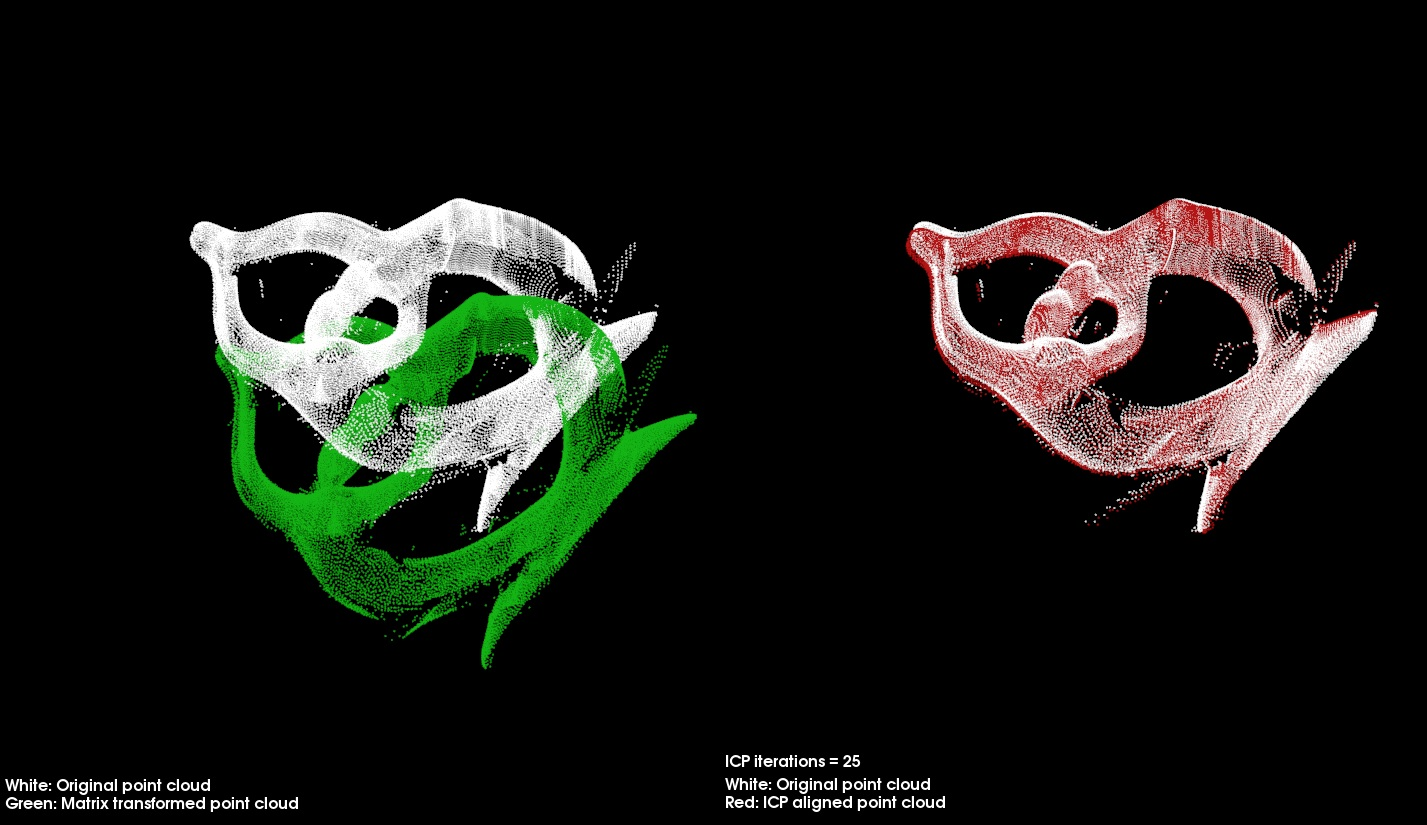
\includegraphics[width=\textwidth]{figures/2016-10-8/icp_result_fish}
	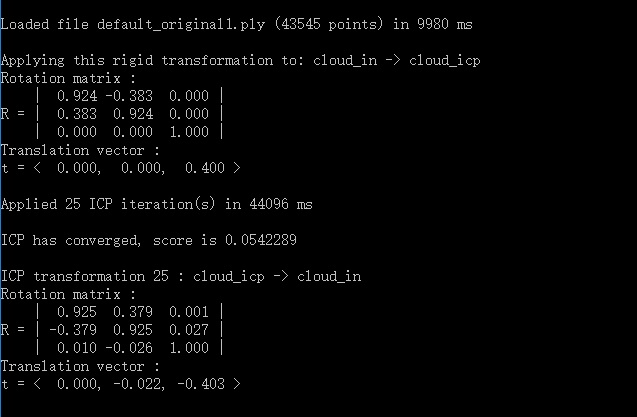
\includegraphics[width=\textwidth]{figures/2016-10-8/icp_result}
	\caption{The results of registration using ICP algorithm.}
\end{figure}